\section{Evaluation}
\label{sec:evaluation}

In this section, we compare {\ProjName} against {\SOAName}, presented in Chapter~\ref{chp:pldi20}.
First, we evaluate the code size reduction achieved by each technique, demonstrating that our approach is on a par with {\SOAName}. Then we show that {\ProjName} reduces significantly the overhead of function merging. % to such a degree that it becomes negligible.
Combined with the speedup in later stages of the compilation pipeline due to the reduced amount of code, {\ProjName} leads to faster end-to-end compilation than a baseline with no function merging enabled. Finally, we demonstrate how our contributions reduce the memory usage by several orders of magnitude. 

\subsection{Experimental Setup}
%We compare {\ProjName}, our novel function merging technique, against {\SOAName}, the  state-of-the-art~\cite{rocha20}.
In addition to evaluating \SOAName, we also consider four variations of our technique based on two dimensions:
1) the linear Pairwise Alignment (PA) versus the quadratic {\NW} Alignment (NW), both on a per basic block manner and
2) using a multi-tier profitability analysis versus using only the standard profitability analysis from {\SOAName}, which is the analysis applied on the whole function after generating the merged function.
As described in Section~\ref{sec:contribution}, the [PA] variant is, by construction, limited to merging only basic blocks of the same size. The [NW] variant can merge blocks of different sizes. The four variations are:

\begin{itemize}
    \item {[PA]}: PA with the Multi-tier Profitability analysis.
    \item {[PA,NMP]}: PA with No Multi-tier Profitability.
    \item {[NW]}: NW with the Multi-tier Profitability.
    \item {[NW,NMP]}: NW with No Multi-tier Profitability.
    %\item {[NW,SS]}: NW with Block Profitability but applied on blocks of the Same Size (SS).
\end{itemize}

%For \SOAName, we used the version published in their evaluation artifact~\cite{SalSSA}.
To keep the comparison fair, we implemented {\ProjName} for the same compiler as \SOAName, LLVM \fixme{v11}. We evaluated all techniques on the C/C++ programs from the SPEC CPU 2006 and the SPEC CPU 2017 benchmark suites~\cite{spec}. The baseline in all cases is the LLVM build in full LTO mode without any function merging.

We target the Intel x86 architecture.
All experiments were performed on a dedicated server with a quad-core Intel Xeon CPU E5-2650, 64 GiB of RAM, running Ubuntu 18.04.3 LTS. To minimize the effect of measurement noise, we repeated all compilation and runtime overhead experiments 5 times. We report the average values and their 95\% confidence intervals.

We evaluate all approaches in terms of code size reduction, time overhead of function merging, end-to-end compilation time, and peak memory usage. To better examine the trade-off between code size reduction and compilation time, we also introduce and measure a new metric called \textit{average reduction speed} which shows the efficiency of the optimization at reducing code size. This metric offers a single number that allows us to compare how different versions address the trade-off between compilation time and code size reduction.

\begin{definition}[Average Reduction Speed]
For a given input program and optimization, let $S$ and $S_0$ be the size of the program with and without the given optimization, respectively.
$R = S_0 - S$ represents the reduction achieved by such optimization.
Let $T$ be the running time of the optimization pass.
We define the \textit{average reduction speed} as:
\[
   ARS = \frac{R}{T}
\]  
\end{definition}

\subsection{Code Size Reduction} \label{sec:eval:size}

Figures~\ref{fig:size-reduction-both} reports the reduction on the size of the linked object files produced by the compiler.
While limiting alignment at a basic block granularity seems restrictive, its effect on code size is small. Even the worst performing variants of {\ProjName} are still within 3 percentage points of {\SOAName}, while both [PA] and [NW] achieve good results that are on a par with {\SOAName}. [PA]'s code size reduction varies from 5 percentage points worse to over 10 points better than {\SOAName}. On average, it is within 1 percentage point of the reduction achieved by {\SOAName}. [NW] almost always achieves better code size reduction than [PA] and on average outperforms {\SOAName} by a small margin. Since our primary aim is to reduce the high compile-time overheads of {\SOAName}
%, in the following sections,
a small loss of code reduction is acceptable. 

 \begin{figure}[h]
   \centering
 \begin{subfigure}{\textwidth}
 \center
   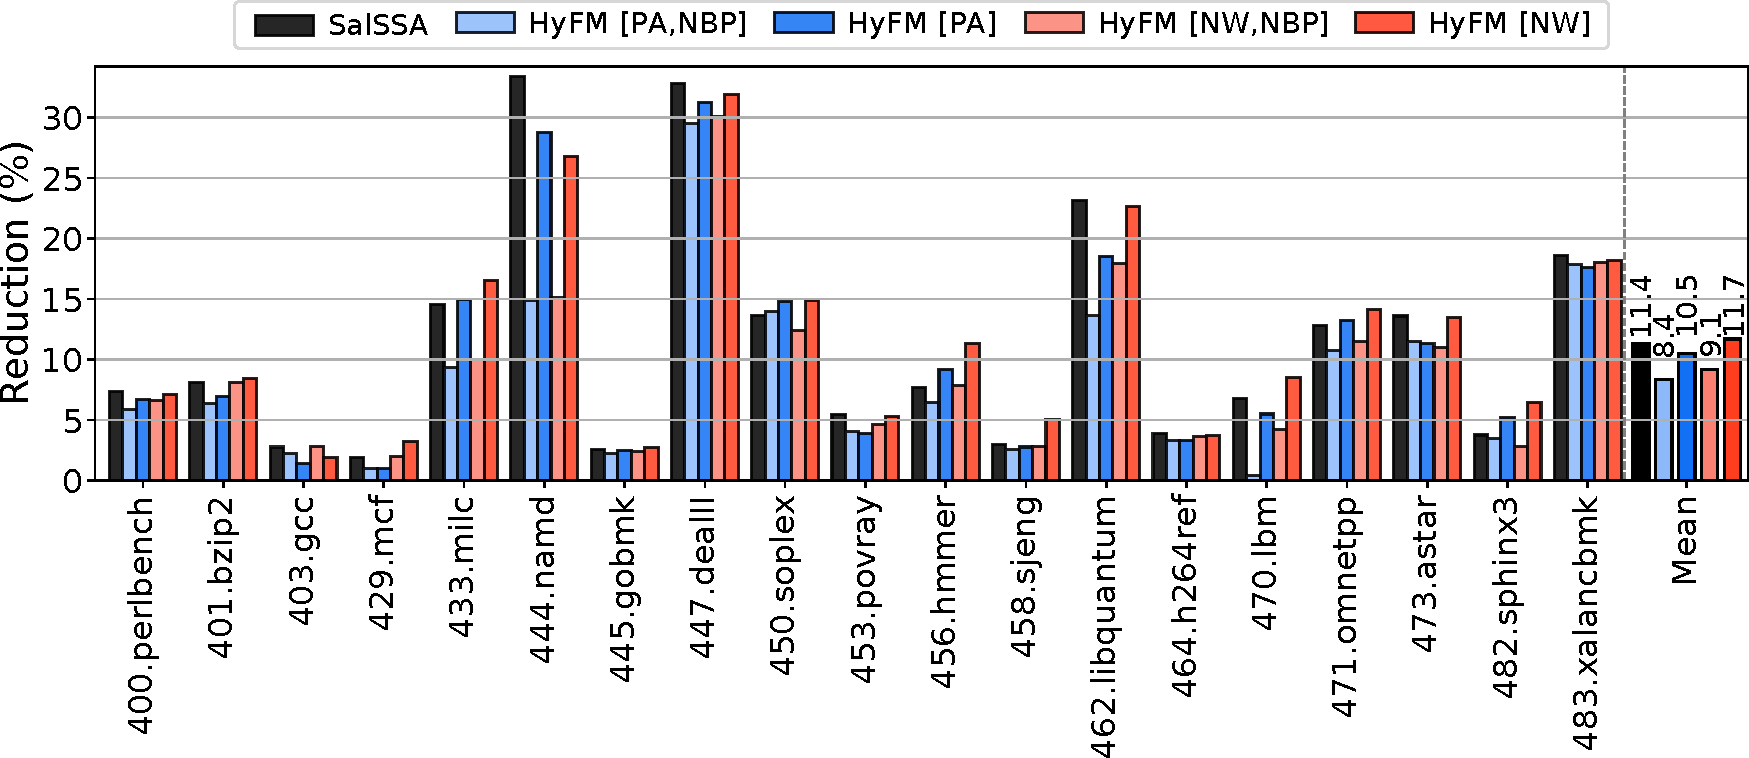
\includegraphics[width=\textwidth]{src/lctes21/figs/reduction-spec06.pdf}
 \caption{SPEC CPU 2006.}
 \label{fig:size-reduction-spec06}
 \end{subfigure}
 \\
 \begin{subfigure}{\textwidth}
 \center
   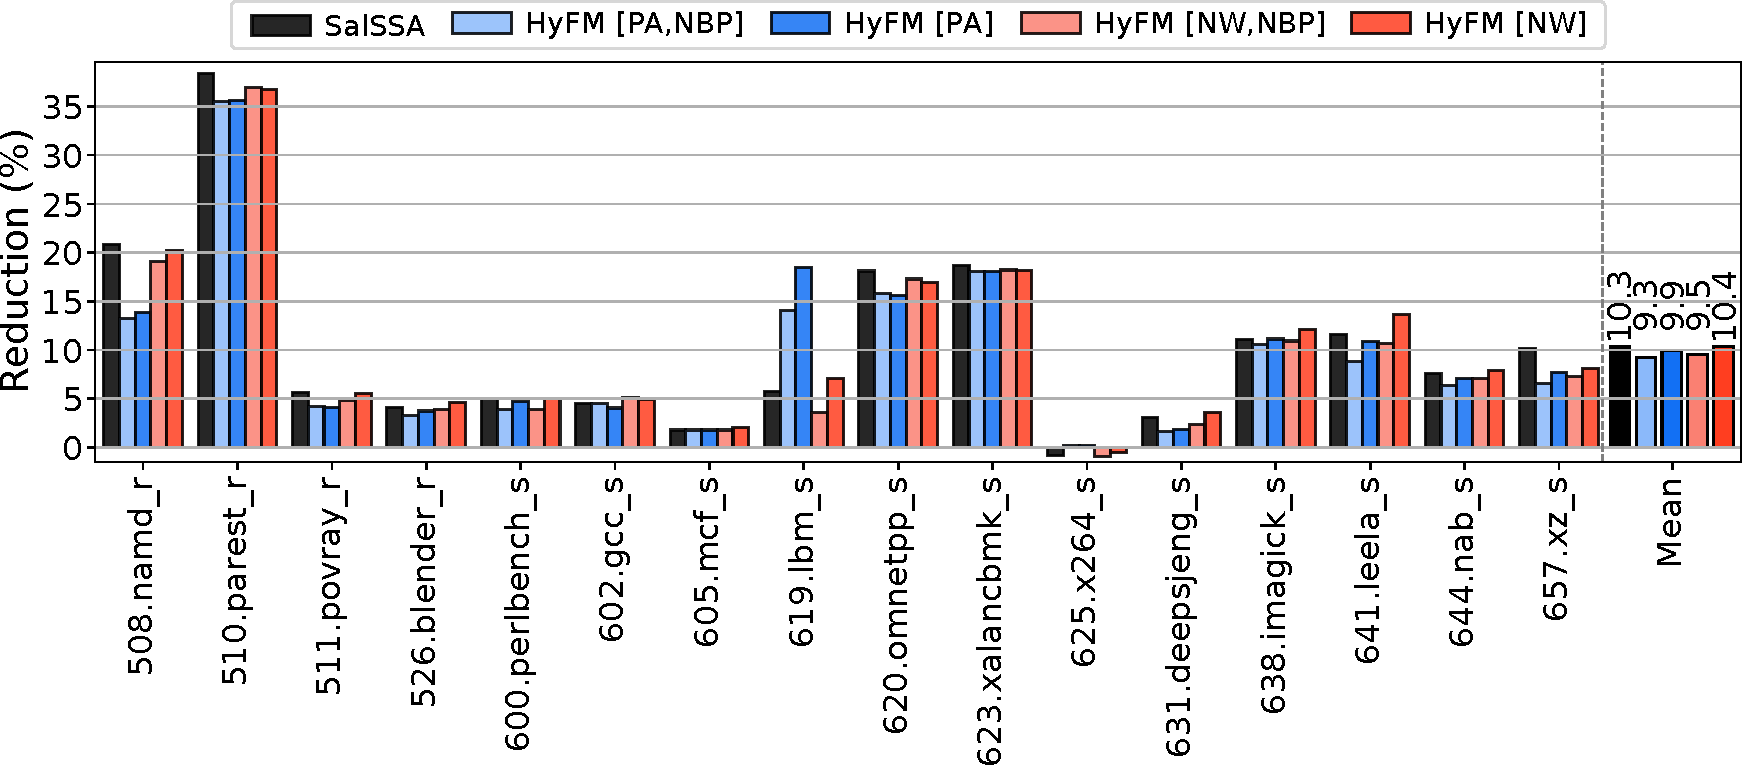
\includegraphics[width=\textwidth]{src/lctes21/figs/reduction-spec17.pdf}
 \caption{SPEC CPU 2017.}
 \label{fig:size-reduction-spec17}
 \end{subfigure}
 \caption{Linked object size reduction over LLVM LTO
      when performing function merging with {\ProjName} or {\SOAName} on SPEC CPU 2006 and 2017. On average, {\ProjName} improves code size reduction.}
  \label{fig:size-reduction-both}
 \end{figure}

%\begin{figure*}[t]
%  \centering
%  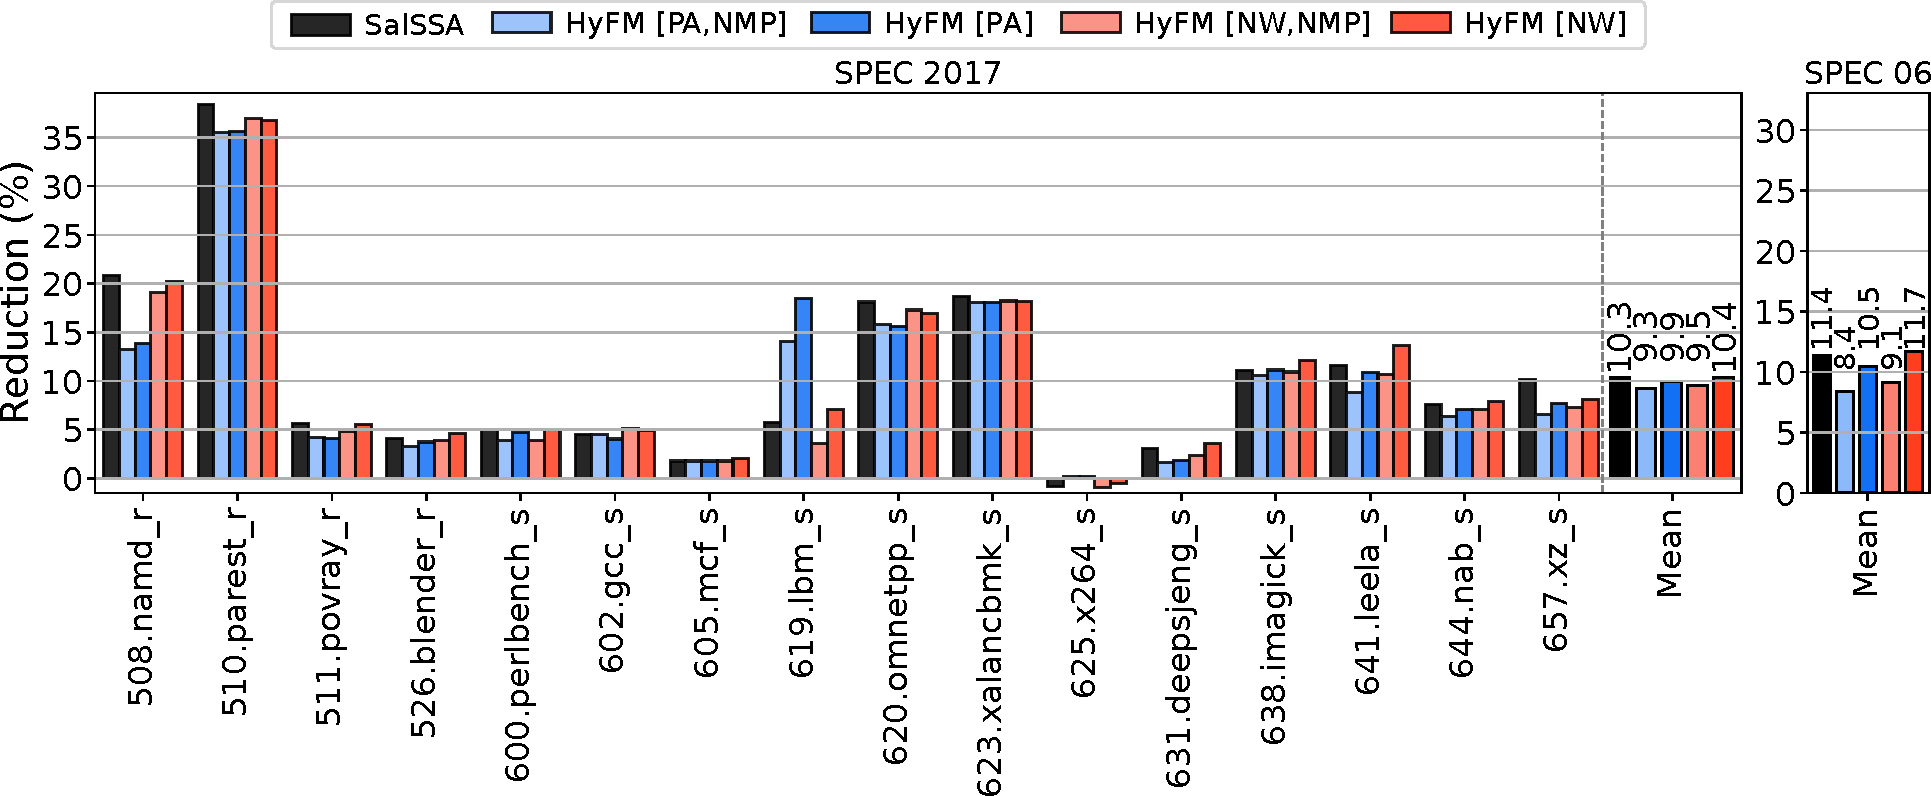
\includegraphics[width=0.95\linewidth]{src/lctes21/figs/reduction-spec17-06.pdf}
%  \caption{Linked object size reduction over LLVM LTO
%      when performing function merging with {\ProjName} or {\SOAName} on SPEC CPU 2006 and 2017. On average, {\ProjName} improves code size reduction.}
%  \label{fig:size-reduction-both}
%\end{figure*}

%Overall, {\ProjName} is on a par with the state of the art {\SOAName}.
%Since our primary aim is to reduce the high compile-time overheads of function merging, as described in Sections~\ref{sec:eval:compilation-time} and \ref{sec:eval:memory}, a small loss of code size reduction is acceptable.

%Even though restricting merging exclusively to basic blocks of the same size seems, at first glance, excessively strong, its effect on code size reduction is limited. On average, same size blocks lead to less than 1\% change compared to the state of the art.

These results indicate that the multi-tier profitability analysis is the single most important component of our approach. 
The two variants without the multi-tier profitability analysis, [PA,NMP] and [NW,NMP], are consistently worse than their counterparts that include this analysis, i.e. [PA] and [NW]. The multi-tier analysis contributes on average about 1 percentage point in code reduction for SPEC 2017 and more than 2 points for SPEC 2006.
The multi-tier profitability analysis has an important impact in the quality of the merged function.
While {\SOAName} lets unprofitable merged subsequences through as long as they are outweighed by profitable subsequences elsewhere in the merged function, {\ProjName} filters such unprofitable subsequences out.

The next most important effect comes from the choice of alignment algorithm. {\NW} is on average half a percentage point better than Pairwise Alignment for SPEC 2017 and about one percentage point better for SPEC 2006. Given that Pairwise Alignment only aligns blocks of the same size and does not try to discover optimal alignments, this difference is smaller than one would expect.
It indicates that profitable pairs of basic blocks tend to be extremely similar if not identical, as discussed in Section~\ref{sec:motivation}.
Still, {\NW} results in more size reduction.
When code size reduction is paramount, [NW] might be a better choice than [PA], but as we will see in Sections~\ref{sec:eval:compilation-time} and \ref{sec:eval:memory}, there is still a trade-off to navigate.

We get the biggest improvement by {[PA]} compared to {\SOAName} and {[NW]} for \texttt{lbm}, where it reduces the program's object file by 18.5\%, almost 13 percentage points more than the competition.
%%%%%%It's actually merging a few profitable basic blocks while giving up on several unprofitable merge sequences
%This comes from discovering a merging opportunity between two large basic blocks of the same size.
%Both {[PA]} and {[PA,NMP]} try merging these blocks but {\SOAName}, {[NW]}, and {[NW,NMP]} choose to focus on other candidates. Compared to {[PA,NMP]}, {[PA]} also finds and profitably merges the same function as {\SOAName} leading to even higher code size reduction.
{\SOAName} is able to profitably merge two pairs of functions.
On the other hand, {[PA,NMP]} chooses to perform a chained merge of the three largest functions in \texttt{lbm}, resulting in a significantly smaller binary.
This is possible because {[PA,NMP]} is merging some nearly identical pairs of basic blocks of the same size.
With the multi-tier profitability analysis, {[PA]} successfully identifies all four cases. 
{[NW]} fails to identify all of these cases, even though it is still better than {\SOAName}.
This exposes existing limitations in the cost model used by our profitability analysis.
%\fixme{Is this a cost model problem?}

The two worst results for {[PA]} are for the \texttt{namd} benchmark in both SPEC 2006 and SPEC 2017. {\SOAName} achieves close to 7 percentage points more than {[PA]} in code size reduction.
In both cases, Pairwise Alignment limits the number of successful merge operations. The variants using {\NW} recover most of the lost reduction. 

% \begin{figure}[h]
%   \centering
%   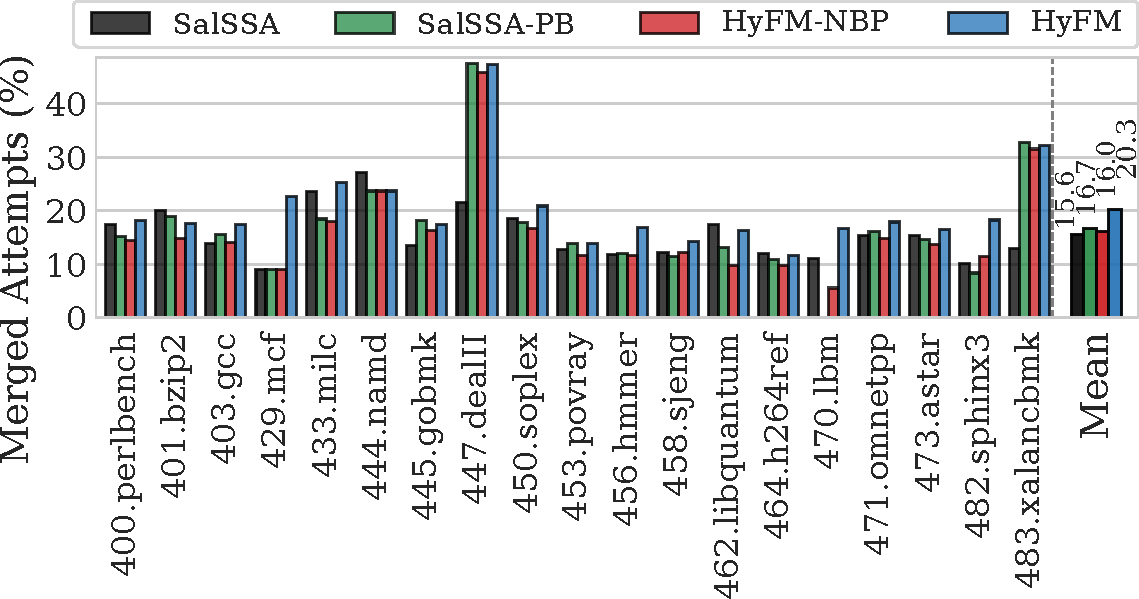
\includegraphics[width=\linewidth]{figs/merged-attempts-perc-spec06.pdf}
%   \caption{Number successful merging attempts on SPEC 2006.}
%   \label{fig:merged-attempts-perc-spec06}
% \end{figure}

% \begin{figure}[h]
%   \centering
%   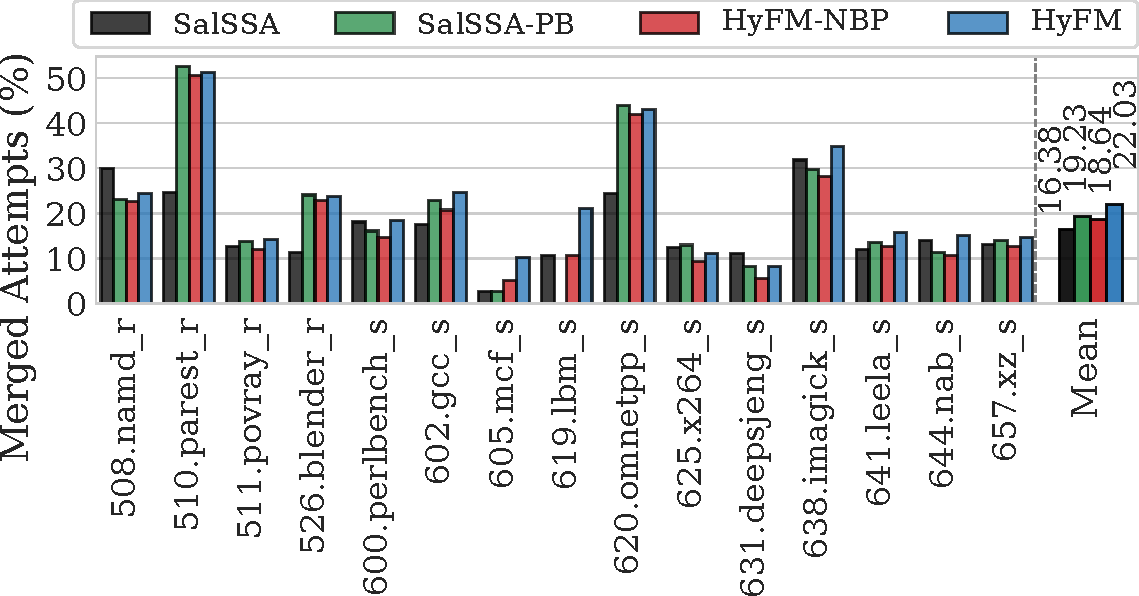
\includegraphics[width=\linewidth]{figs/merged-attempts-perc-spec17.pdf}
%   \caption{Number of successful merging attempts on SPEC 2017.}
%   \label{fig:merged-attempts-perc-spec17}
% \end{figure}

% \begin{figure}[h]
%   \centering
%   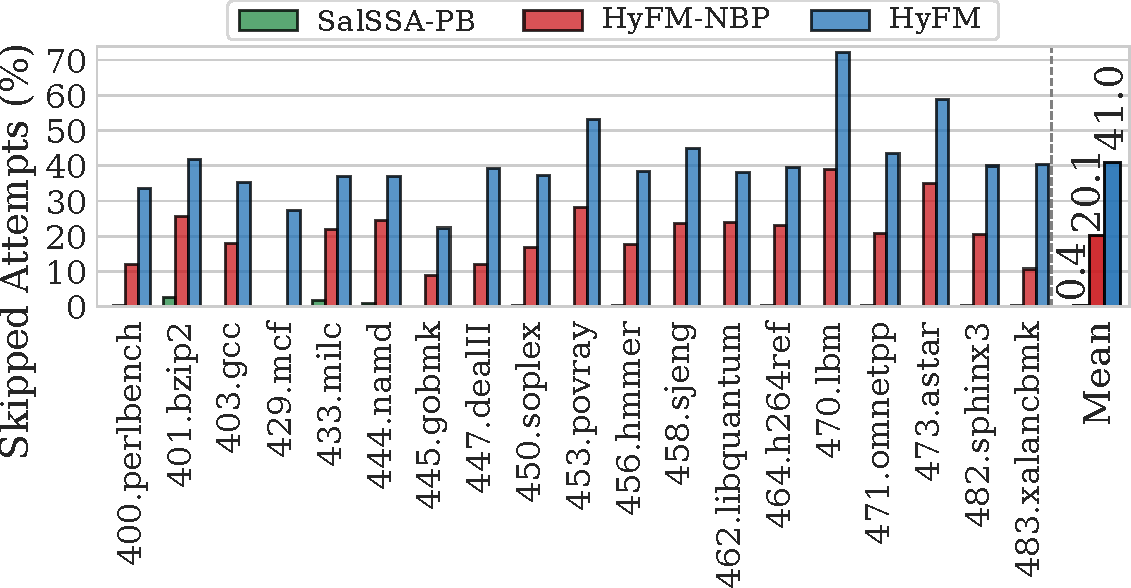
\includegraphics[width=\linewidth]{figs/skipped-attempts-perc-spec06.pdf}
%   \caption{Number of skipped merging attempts on SPEC 2006.}
%   \label{fig:skipped-attempts-perc-spec06}
% \end{figure}

% \begin{figure}[h]
%   \centering
%   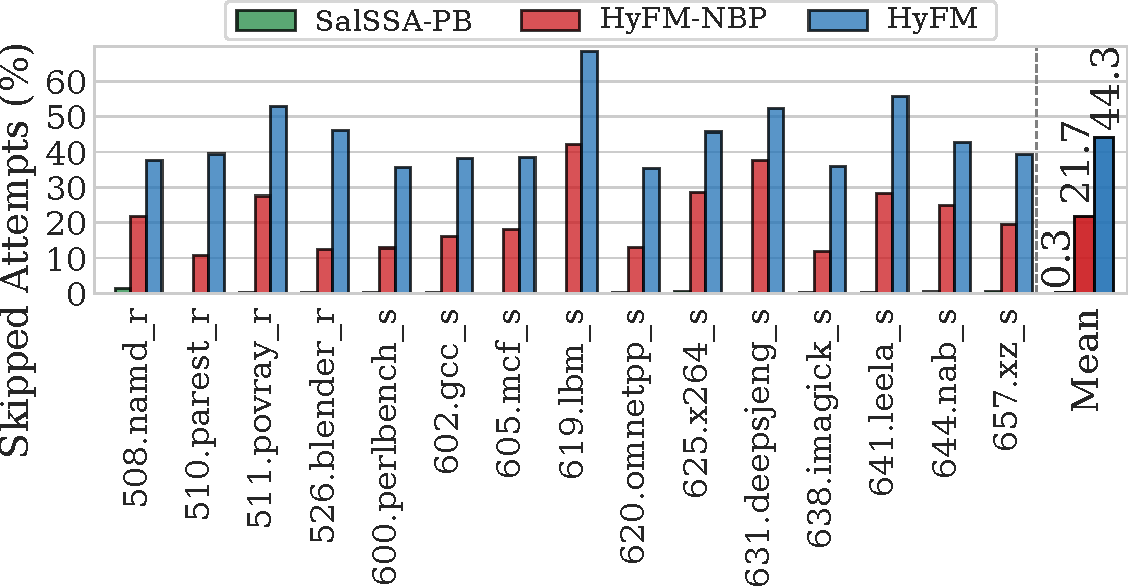
\includegraphics[width=\linewidth]{figs/skipped-attempts-perc-spec17.pdf}
%   \caption{Number of skipped merging attempts on SPEC 2017.}
%   \label{fig:skipped-attempts-perc-spec17}
% \end{figure}


% \begin{figure*}[h]
%   \centering
%   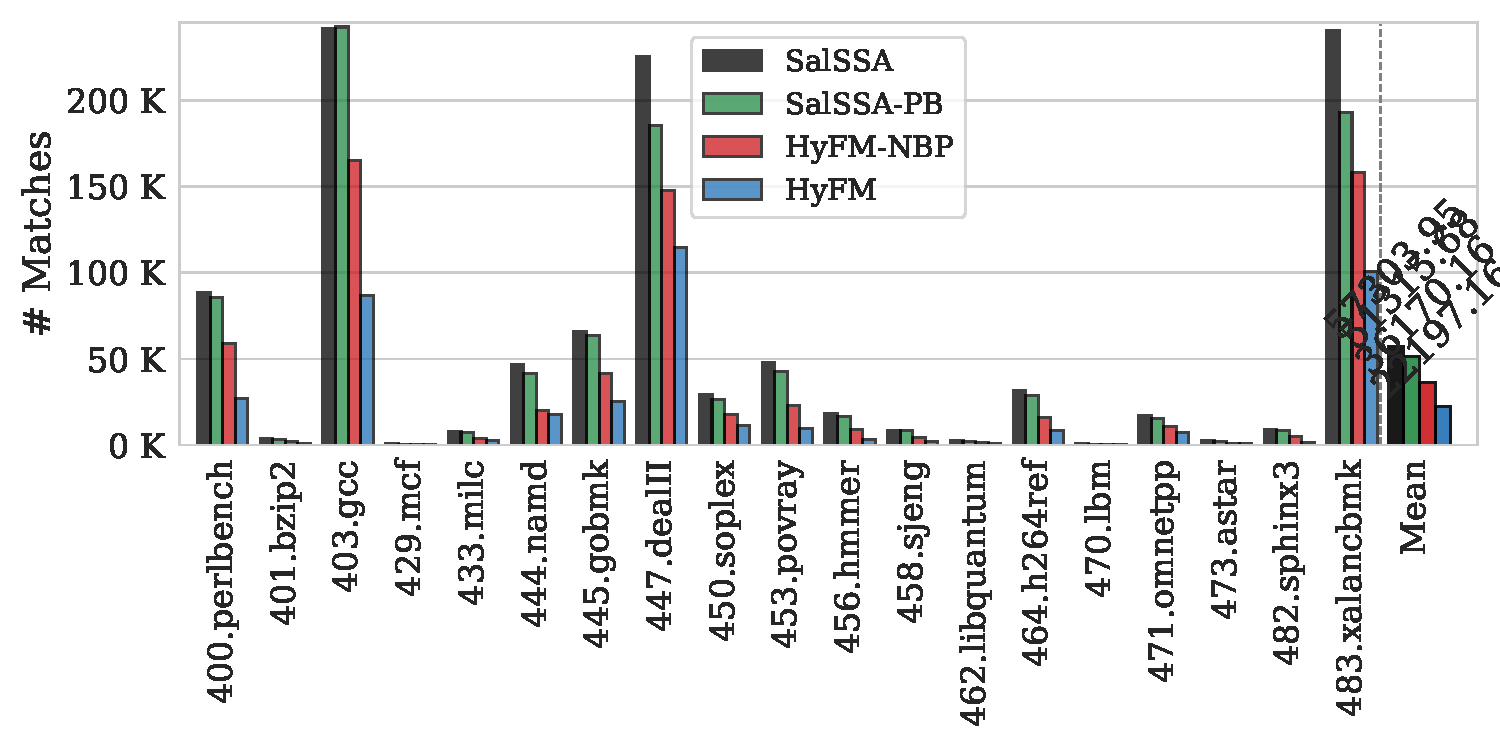
\includegraphics[width=0.85\linewidth]{figs/total-num-matches-spec06.pdf}
%   \caption{Total number of matching entries, including profitable and unprofitable attempts. SPEC 2006.}
%   \label{fig:total-num-matches-spec06}
% \end{figure*}

% \begin{figure*}[h]
%   \centering
%   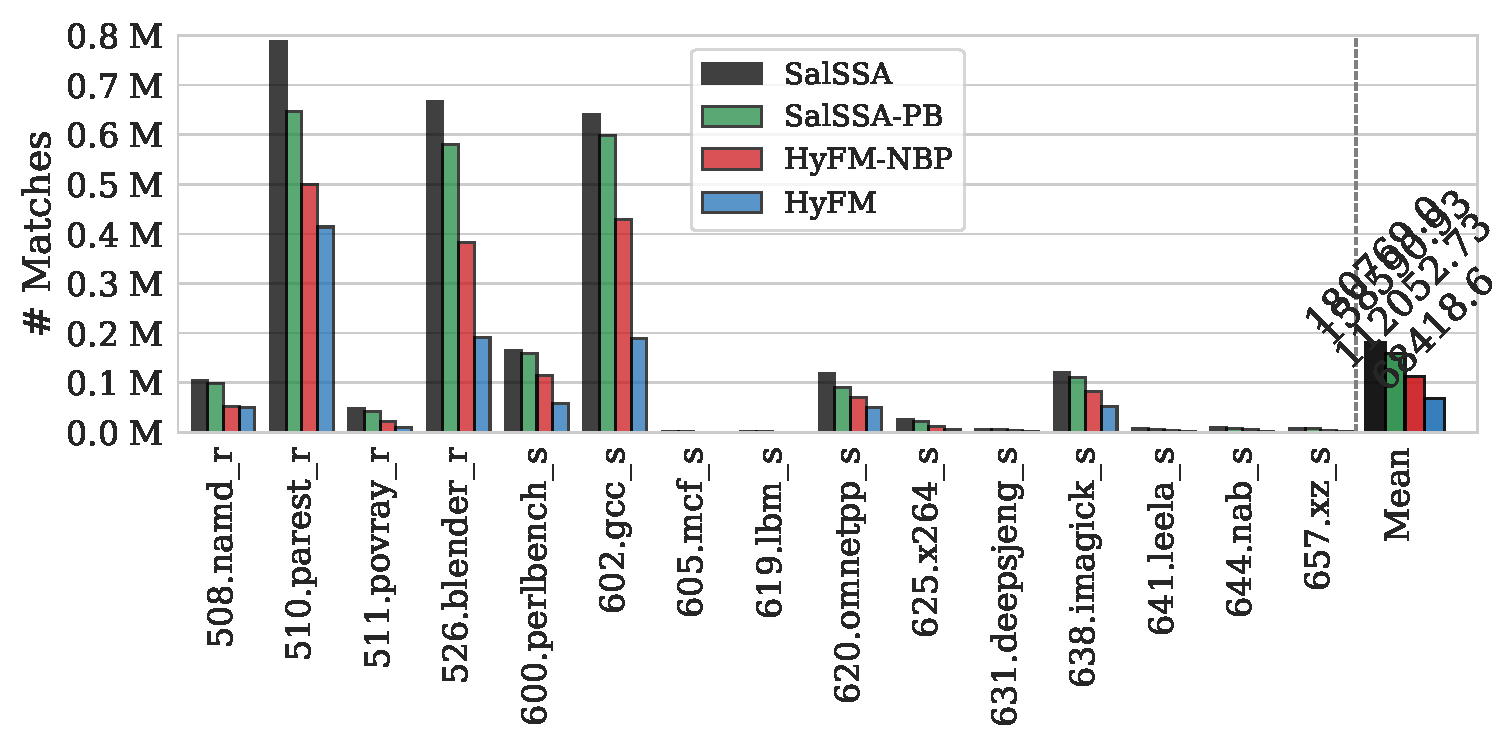
\includegraphics[width=0.85\linewidth]{figs/total-num-matches-spec17.pdf}
%   \caption{Total number of matching entries, including profitable and unprofitable attempts. SPEC 2017.}
%   \label{fig:total-num-matches-spec17}
% \end{figure*}

\subsection{Speeding Up Function Merging} \label{sec:eval:pass-speedup}

 \begin{figure}[h]
   \centering
 \begin{subfigure}{\textwidth}
 \center
   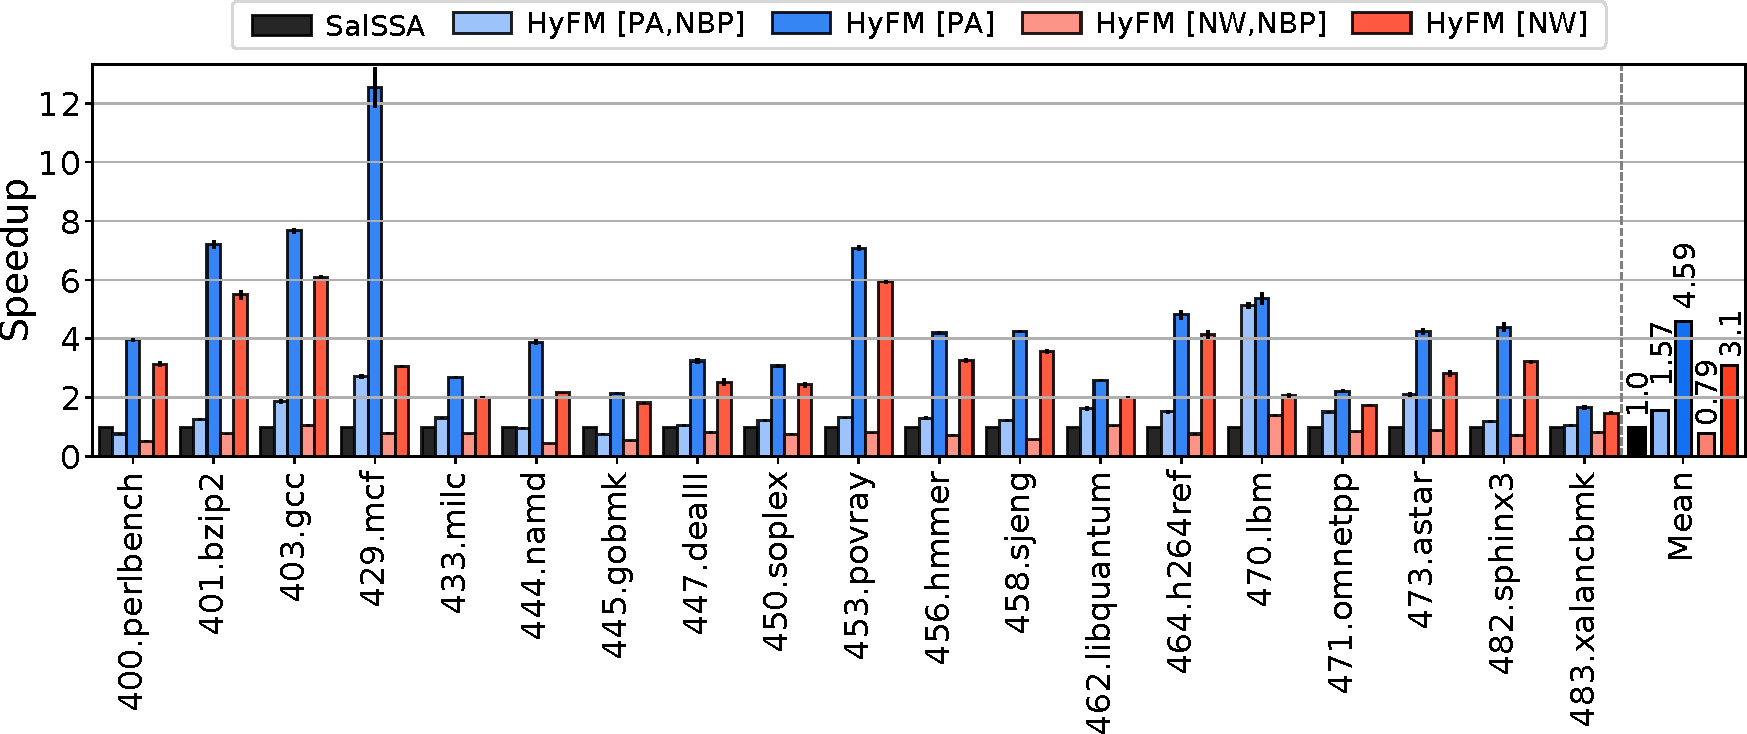
\includegraphics[width=\textwidth]{src/lctes21/figs/speedup-spec06.pdf}
 \caption{SPEC CPU 2006.}
 \label{fig:speedup-spec06}
 \end{subfigure}
 \\
 \begin{subfigure}{\textwidth}
 \center
   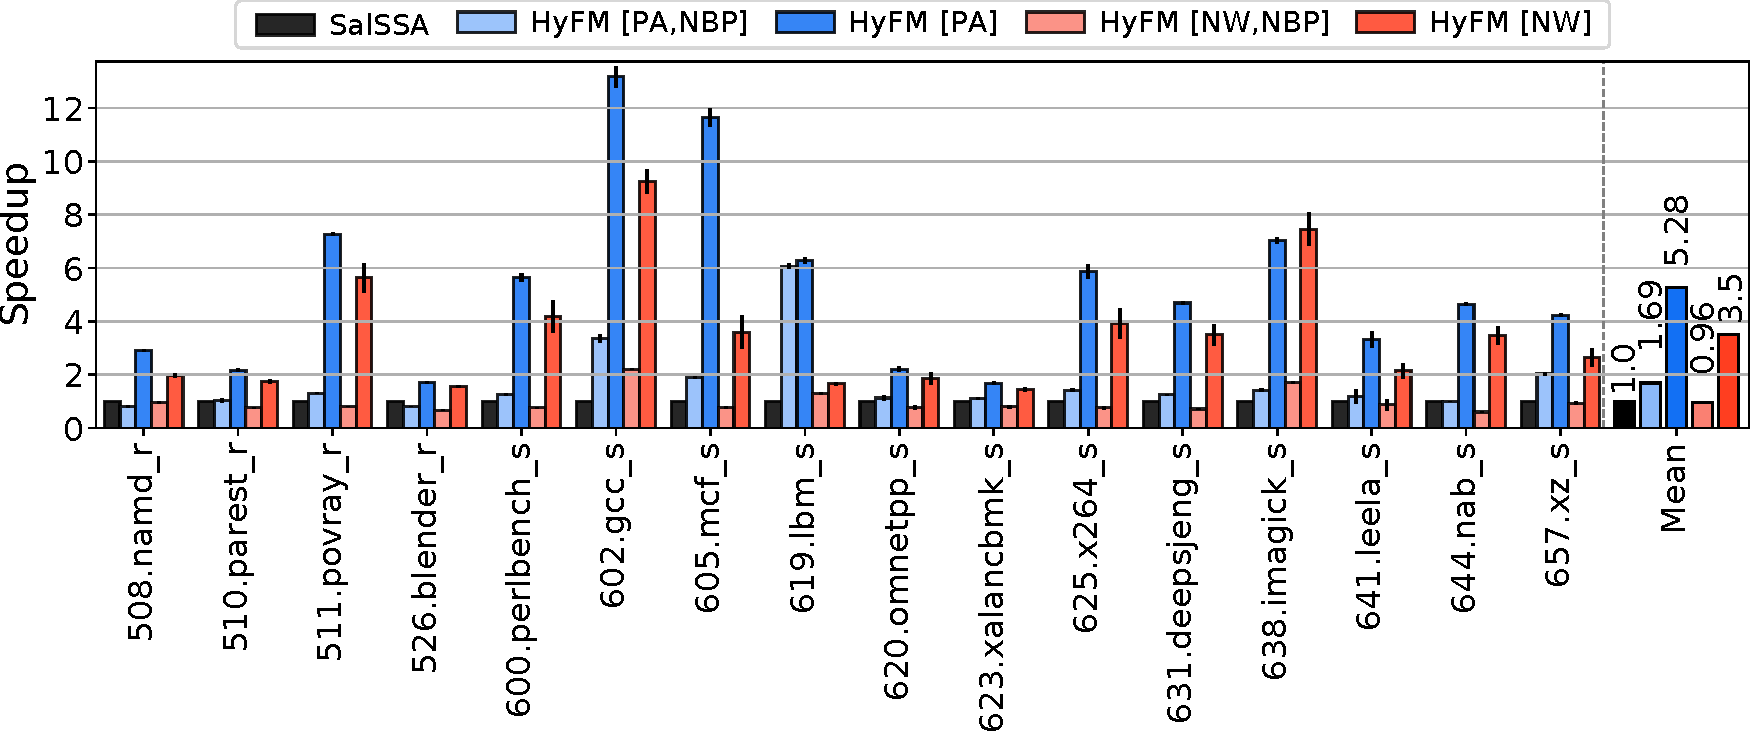
\includegraphics[width=\textwidth]{src/lctes21/figs/speedup-spec17.pdf}
 \caption{SPEC CPU 2017.}
 \label{fig:speedup-spec17}
 \end{subfigure}
 \caption{Speedup of the function merging pass in isolation relative to {\SOAName}. The multi-tier profitability analysis reduces the number of unprofitable merge operations leading to a significant speedup.}
  \label{fig:speedup-both}
 \end{figure}

%\begin{figure*}[t]
%  \centering
%  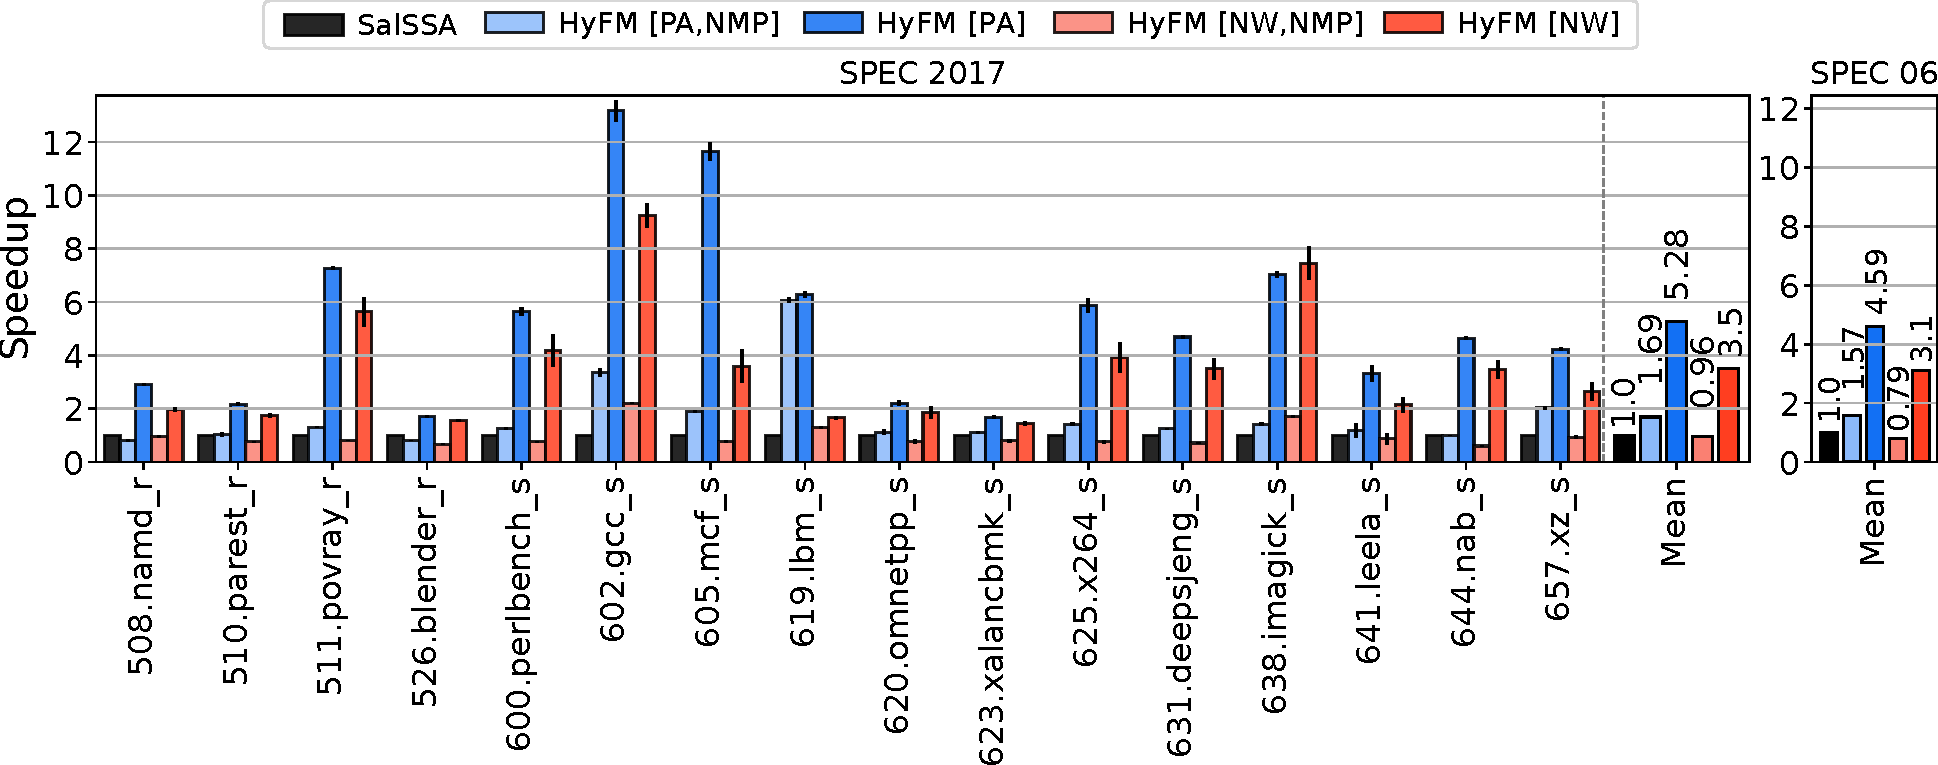
\includegraphics[width=0.95\linewidth]{src/lctes21/figs/speedup-spec17-06.pdf}
%  \caption{Speedup of the function merging pass in isolation relative to {\SOAName}. The multi-tier profitability analysis reduces the number of unprofitable merge operations leading to a significant speedup.}
%  \label{fig:speedup-both}
%\end{figure*}

Figure~\ref{fig:speedup-both} shows the speedup of {\ProjName} relative to {\SOAName}.
This considers only the time taken by the function merging pass, which include all stages discussed in Section~\ref{sec:motivation:breakdown}.
Our novel technique achieves an impressive speedup. For {[PA]} it is on average $5.28\times$ faster for SPEC 2017 and $4.59\times$ for SPEC 2006. Even in the worst case, it achieves a \fixme{50}\% speedup. In the best case, for the SPEC 2017 \texttt{gcc}, function merging under {\ProjName} takes a total of 23.5 seconds instead of 302, which translates to almost $13\times$ less time.

%The two variants with the multi-tier profitability analysis achieve on average three to four times higher speedups than their counterparts without it. This is a direct result of bailing out early. For most benchmarks, only a small number of candidate pairs is profitable. The majority are unprofitable but SalSSA has to merge them anyway to determine their profitability. This is expensive and wasteful. Our approach,on the other hand, is able to estimate profitability early. Only function pairs with any chance of being profitable, that is pairs with at least one profitable pair of basic blocks, move forward to the expensive merge stage.
%The linear pairwise alignment contributes to the performance improvement, too. The variants using pairwise alignment run on average 48% to 98% faster than their Needleman-Wunsch counterparts. The most pronounced case is for lbm where [PA] is around3×faster than [NW]. The blocks paired in lbm are longer than usual, so the quadratic Needleman-Wunsch spends significantly more time trying to align them than our linear pairwise algorithm. Figure 7 shows that the added pairing restrictions from [PA], to focus on blocks with higher similarities, also benefits later stages.
%All components of HyFM contribute towards this result but the multi-tier profitability analysis has the most significant impact. As we show in Figure 7, even though the time spent on the alignment strategy becomes negligible for both [PA,NMP] and [PA], the lack of a multi-tier profitability analysis may degrade the stages associated with code generation. If we accept the alignment for any pair of basic blocks, we may end up producing complex merged functions— code with an excessive amount of branches, phi-nodes,and operand selections — slowing down SSA reconstruction and code simplification. This effect can be observed with [PA,NMP] for many benchmarks in Figure 7. Most notably, for the blender benchmark, [PA,NMP] is slower than SalSSA due to its added pressure on the SSA reconstruction algorithm, even though its alignment strategy runs much faster. For this reason, enabling the multi-tier profitability analysis has a positive impact on later stages.

All components of {\ProjName} contribute towards this result but the multi-tier profitability analysis has the most significant impact. The two variants with the multi-tier profitability analysis achieve on average three to four times higher speedups than their counterparts without it.
To help us understand why, Figure~\ref{fig:breakdown-spec17} shows how the compilation time of each approach is distributed across its various stages. 
Even though the time spent on the alignment strategy becomes negligible with {\ProjName}, the less optimal alignment often produces complex merged functions --- code with an excessive amount of branches, phi-nodes, and operand selections --- slowing down SSA reconstruction and code simplification. This effect is very pronounced for the \texttt{blender} benchmark, where both [PA,NMP] and [NW,NMP] are slower than {\SOAName} due to the added pressure on the SSA reconstruction algorithm, even though the alignment overhead is practically zero.
Similar effects can be observed in other benchmarks.

\begin{figure}[h]
  \centering
  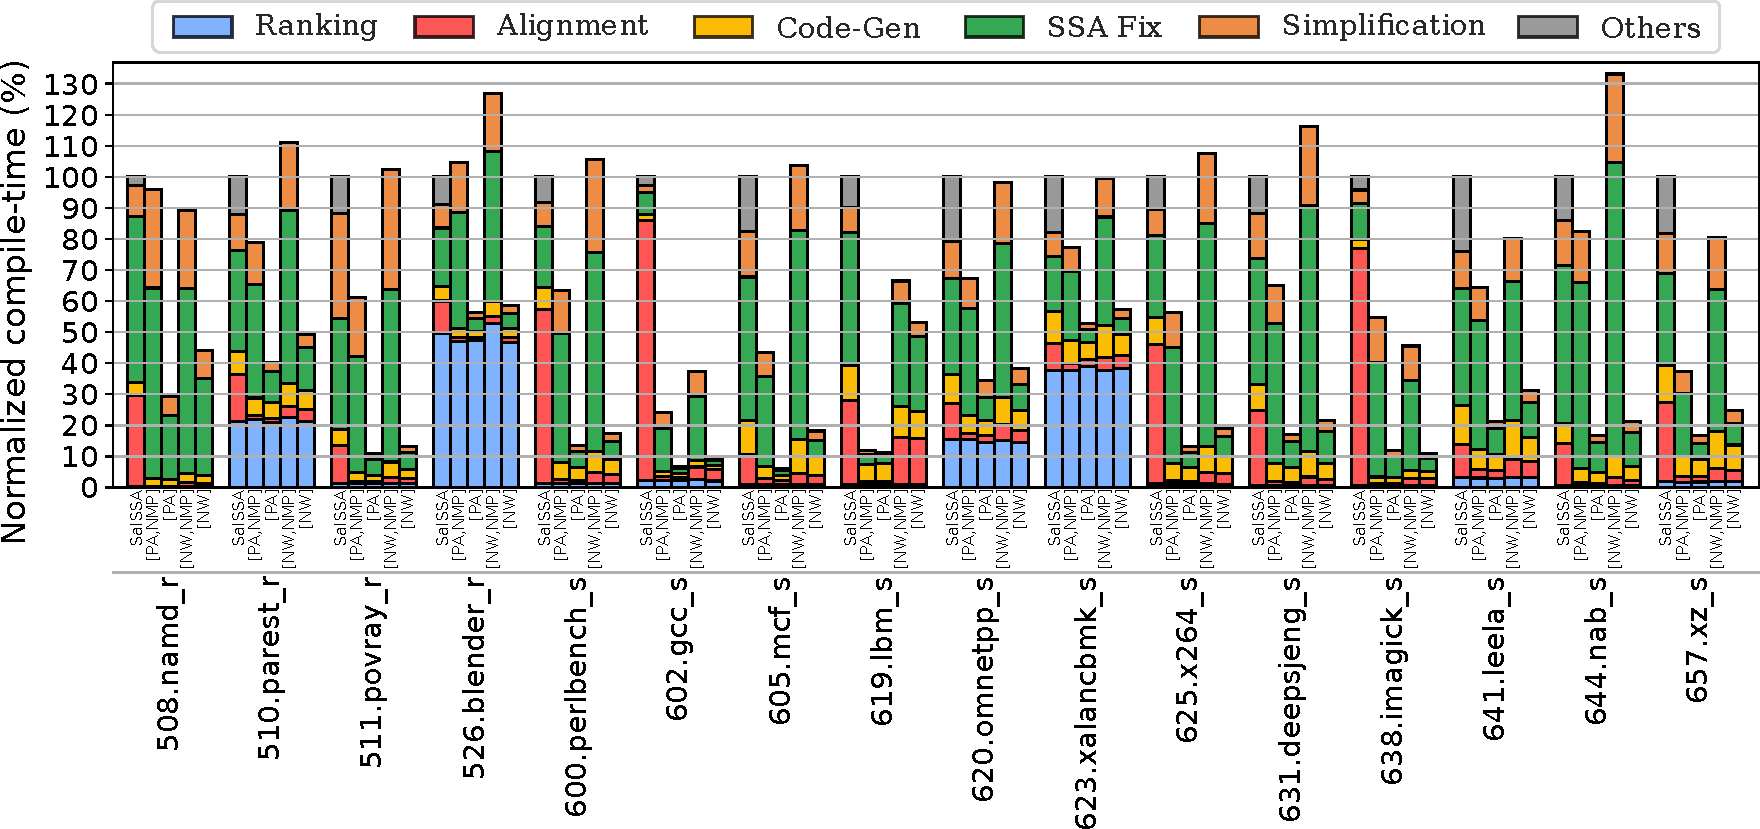
\includegraphics[width=\linewidth]{src/lctes21/figs/breakdown-full-spec17.pdf}
  \caption{Breakdown of the relative runtime for the different stages of the function merging pass. All measurements are normlized by \SOAName's total runtime on the corresponding benchmark. For every benchmark, we show {\SOAName}, [PA,NMP], [PA], [NW,NMP], and [NW], in this order. }
  \label{fig:breakdown-spec17}
\end{figure}

Enabling the multi-tier profitability analysis counters this effect by focusing code generation exclusively on profitable blocks and functions. Most of the complex basic blocks {\ProjName} generates are not profitable for the same reason it is expensive to process them. First-tier profitability filters them out. On top of that, most paired functions under either {\SOAName} or {\ProjName} are unprofitable. {\SOAName} has to merge them anyway to determine their profitability. This is expensive and wasteful. Our approach, on the other hand, is able to estimate profitability early. Only function pairs with any chance of being profitable, that is pairs with at least one profitable pair of basic blocks, move forward to the expensive merge stage.

The linear pairwise alignment contributes to the performance improvement, too. The variants using pairwise alignment run on average 48\% to 98\% faster than their {\NW} counterparts.
%The most pronounced case is for \texttt{mcf} where {[PA]} is approximately $3\times$ faster than {[NW]}. Candidate basic block pairs in \texttt{mcf} are longer than usual, so the quadratic {\NW} spends significantly more time trying to align them than our linear pairwise algorithm. 
The most pronounced case is for \texttt{lbm} where {[PA]} is around $3\times$ faster than {[NW]}. The blocks paired in \texttt{lbm} are longer than usual, so the quadratic {\NW} spends significantly more time trying to align them than our linear pairwise algorithm.
Figure~\ref{fig:breakdown-spec17} shows that the added pairing restrictions from [PA], to focus on blocks with higher similarities, also benefits later stages.

\subsection{End-to-End Compilation Time} \label{sec:eval:compilation-time}

We have also analyzed separately the end-to-end compilation time because reducing code size through function merging has knock-on effects in later stages of the compilation pipeline.
The first order effect is that reducing the number of functions tends to reduce compilation time.
This is not guaranteed though, because merged functions may be more complex, potentially slowing down later compiler analyses and transformations.
Moreover, the time spent merging functions may be so large that it negates any benefits from having fewer functions later in the pipeline.

Even though on a few occasions {\SOAName} reduces end-to-end compilation time, in general, its overhead is large enough to result in an overall compilation time slowdown, 9.5\% to 4.1\% for SPEC 2017 and 2006 respectively.
In contrast, {\ProjName} is so much faster that its compilation time overhead is matched or outweighed by the speedup in later stages. 
This reduction is marginal for SPEC 2017, but for SPEC 2006 {[PA]} reduces the average compilation time by 2.3\% and {[NW]} by 1.6\%.
There is only a single case where {[PA]} results in a significant end-to-end slowdown, 10\% for \texttt{blender}.
%While this is still an improvement compared to {\SOAName}, \fixme{EXPLAIN}.
Figure~\ref{fig:breakdown-spec17} shows that, although [PA] runs faster than {\SOAName}, both of them spent a significant amount of time ranking the function candidates, due to its large number of functions.
Ranking alone in this case takes around 70 seconds. %However, this is beyond the scope of this paper.

Overall, we believe that this reduction in end-to-end compilation time is a very important result. While {\ProjName} is still achieving code-size reduction on par with the state-of-the-art, it does not have the detrimental effects of {\SOAName} on the overall compilation process and can be safely applied.

 \begin{figure}[h]
   \centering
 \begin{subfigure}{\textwidth}
 \center
   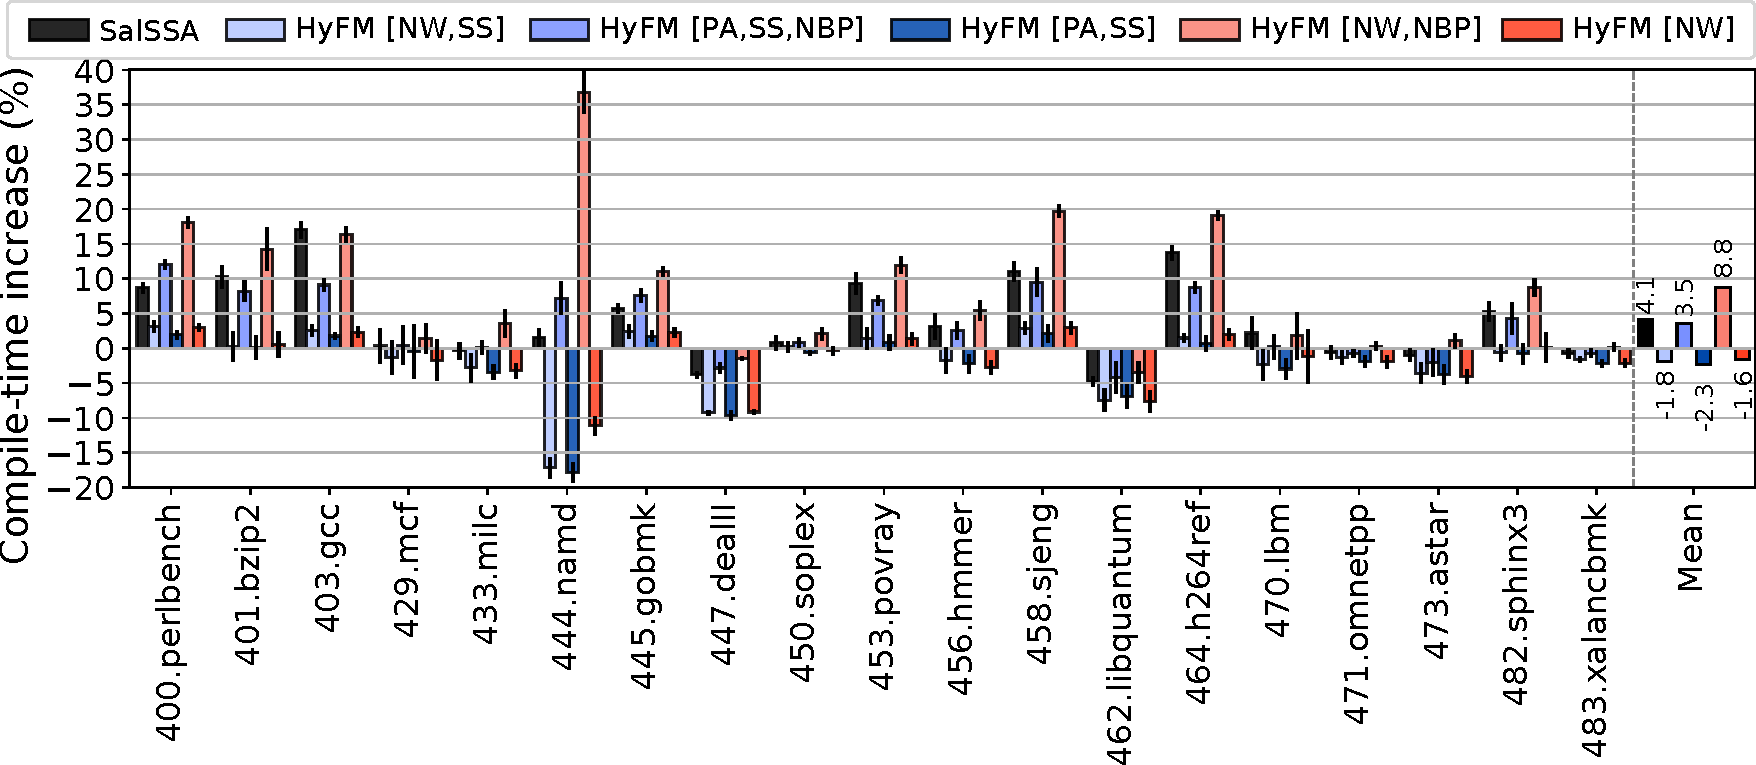
\includegraphics[width=\textwidth]{src/lctes21/figs/compiletime-spec06.pdf}
 \caption{SPEC CPU 2006.}
 \label{fig:compiletime-spec06}
 \end{subfigure}
 \\
 \begin{subfigure}{\textwidth}
 \center
   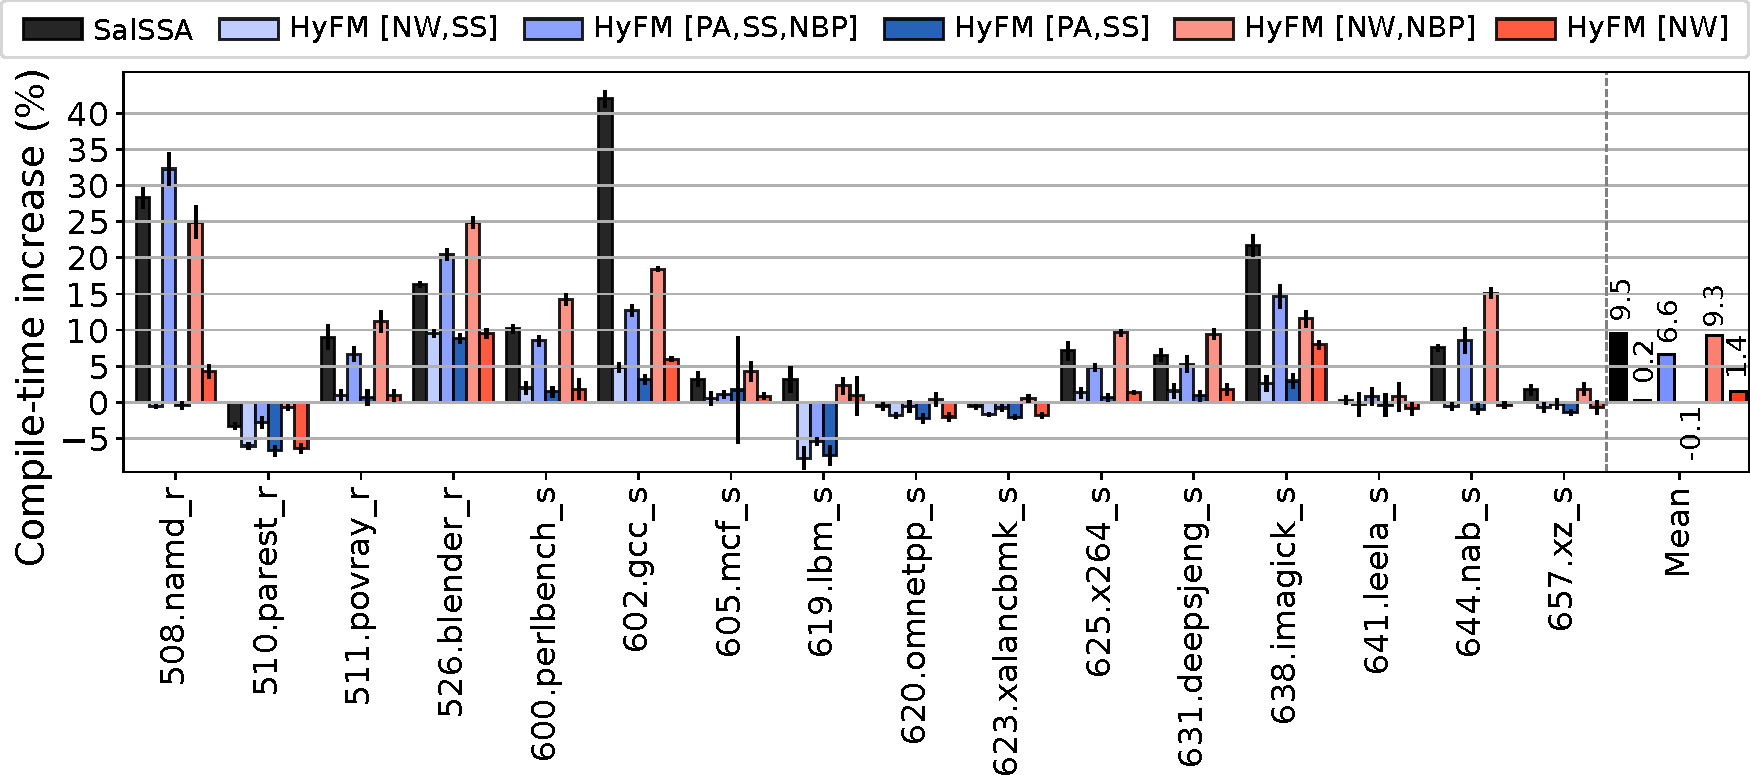
\includegraphics[width=\textwidth]{src/lctes21/figs/compiletime-spec17.pdf}
 \caption{SPEC CPU 2017.}
 \label{fig:compiletime-spec17}
 \end{subfigure}
 \caption{Normalized end-to-end compilation time for SPEC 2017 and SPEC 2006 relative to LLVM LTO.}
  \label{fig:compiletime-both}
 \end{figure}

%\begin{figure*}[h]
%  \centering
%  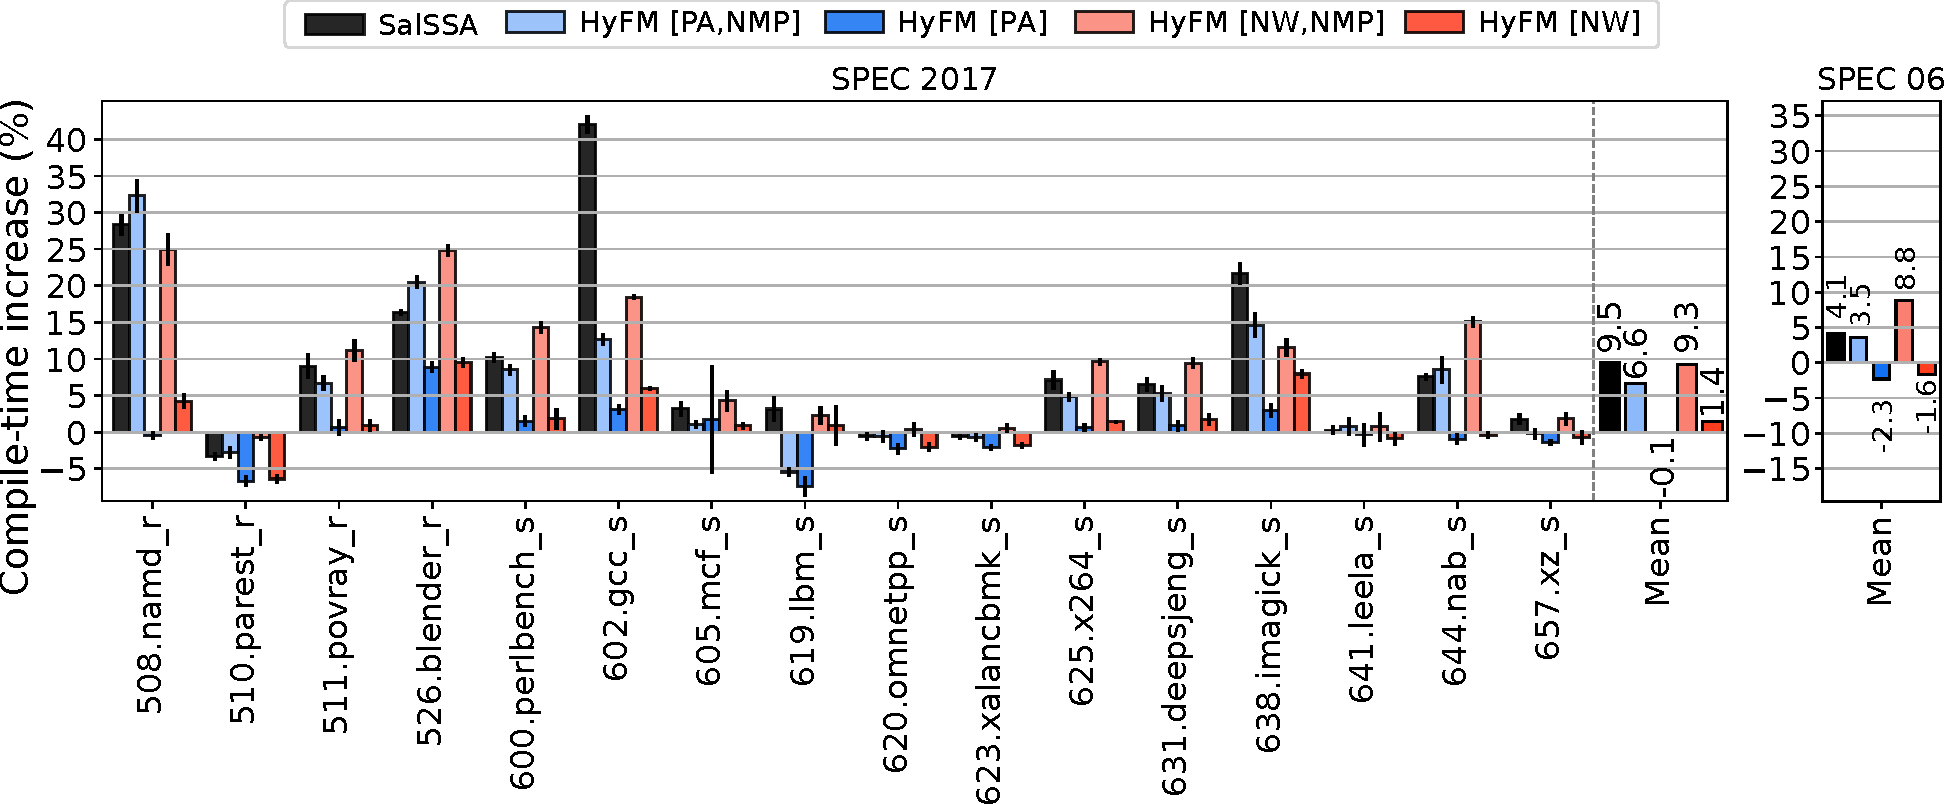
\includegraphics[width=0.95\linewidth]{src/lctes21/figs/compiletime-spec17-06.pdf}
%  \caption{Normalized end-to-end compilation time for SPEC 2017 and SPEC 2006 relative to LLVM LTO.}
%  \label{fig:compilation-both}
%\end{figure*}


\subsection{Code Size and Compilation Time Trade-Off} \label{sec:eval:trade-off}

While the multi-tier profitability analysis improves both code-size reduction and compilation speed, the choice of alignment algorithm introduces a trade-off. Pairwise alignment is better for speed, {\NW} is better for code-size reduction. 
In terms of compilation efficiency, i.e. how much code size reduction we get for the effort we put in, the picture is clearer. In Figure~\ref{fig:ars-both}, the \textit{average reduction speed} suggests that {[PA]} achieves the ideal trade-off, with an average reduction speed of 115.3~KB/s, which is around $3\times$ greater than {\SOAName}'s and 20\% to 40\% greater than [NW].


 \begin{figure}[h]
   \centering
 \begin{subfigure}{\textwidth}
 \center
   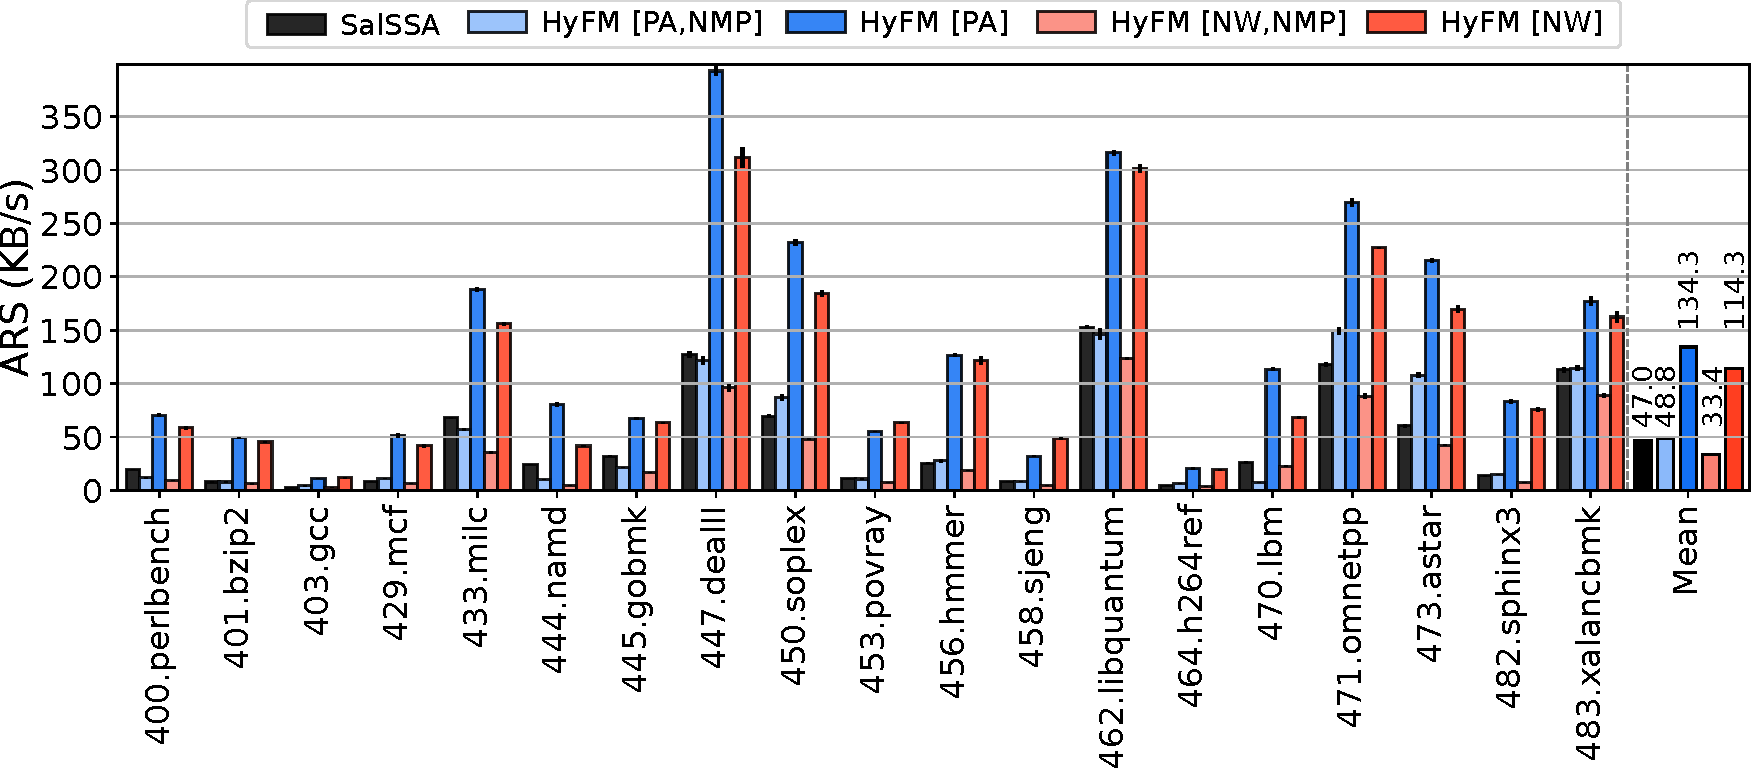
\includegraphics[width=\textwidth]{src/lctes21/figs/ars-spec06.pdf}
 \caption{SPEC CPU 2006.}
 \label{fig:ars-spec06}
 \end{subfigure}
 \\
 \begin{subfigure}{\textwidth}
 \center
   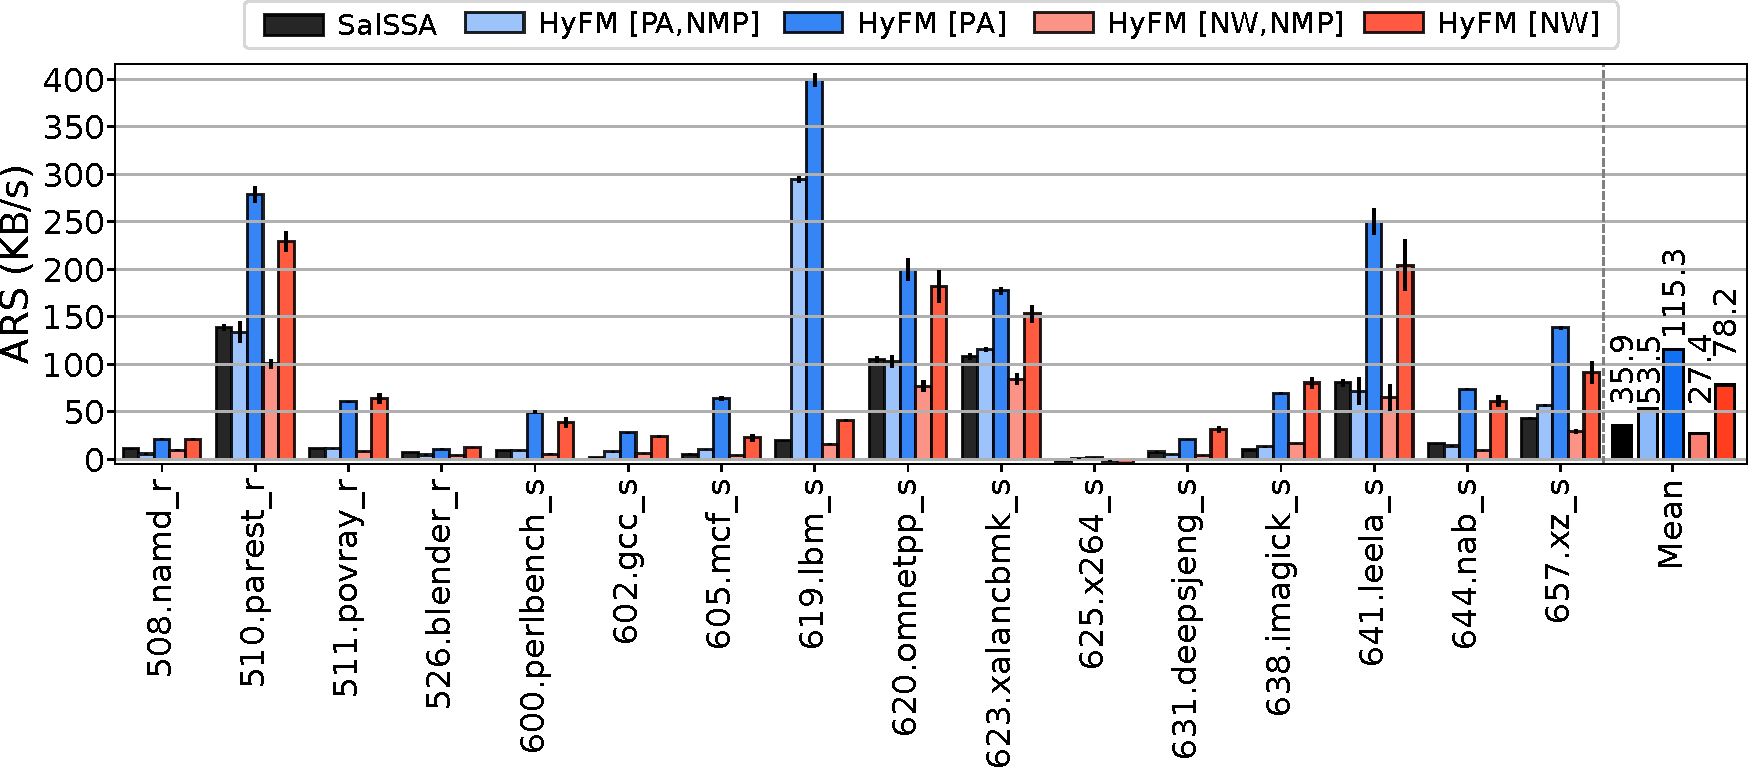
\includegraphics[width=\textwidth]{src/lctes21/figs/ars-spec17.pdf}
 \caption{SPEC CPU 2017.}
 \label{fig:ars-spec17}
 \end{subfigure}
 \caption{Average reduction speed on both SPEC 2006 and 2017.}
  \label{fig:ars-both}
 \end{figure}

%\begin{figure*}[h]
%  \centering
%  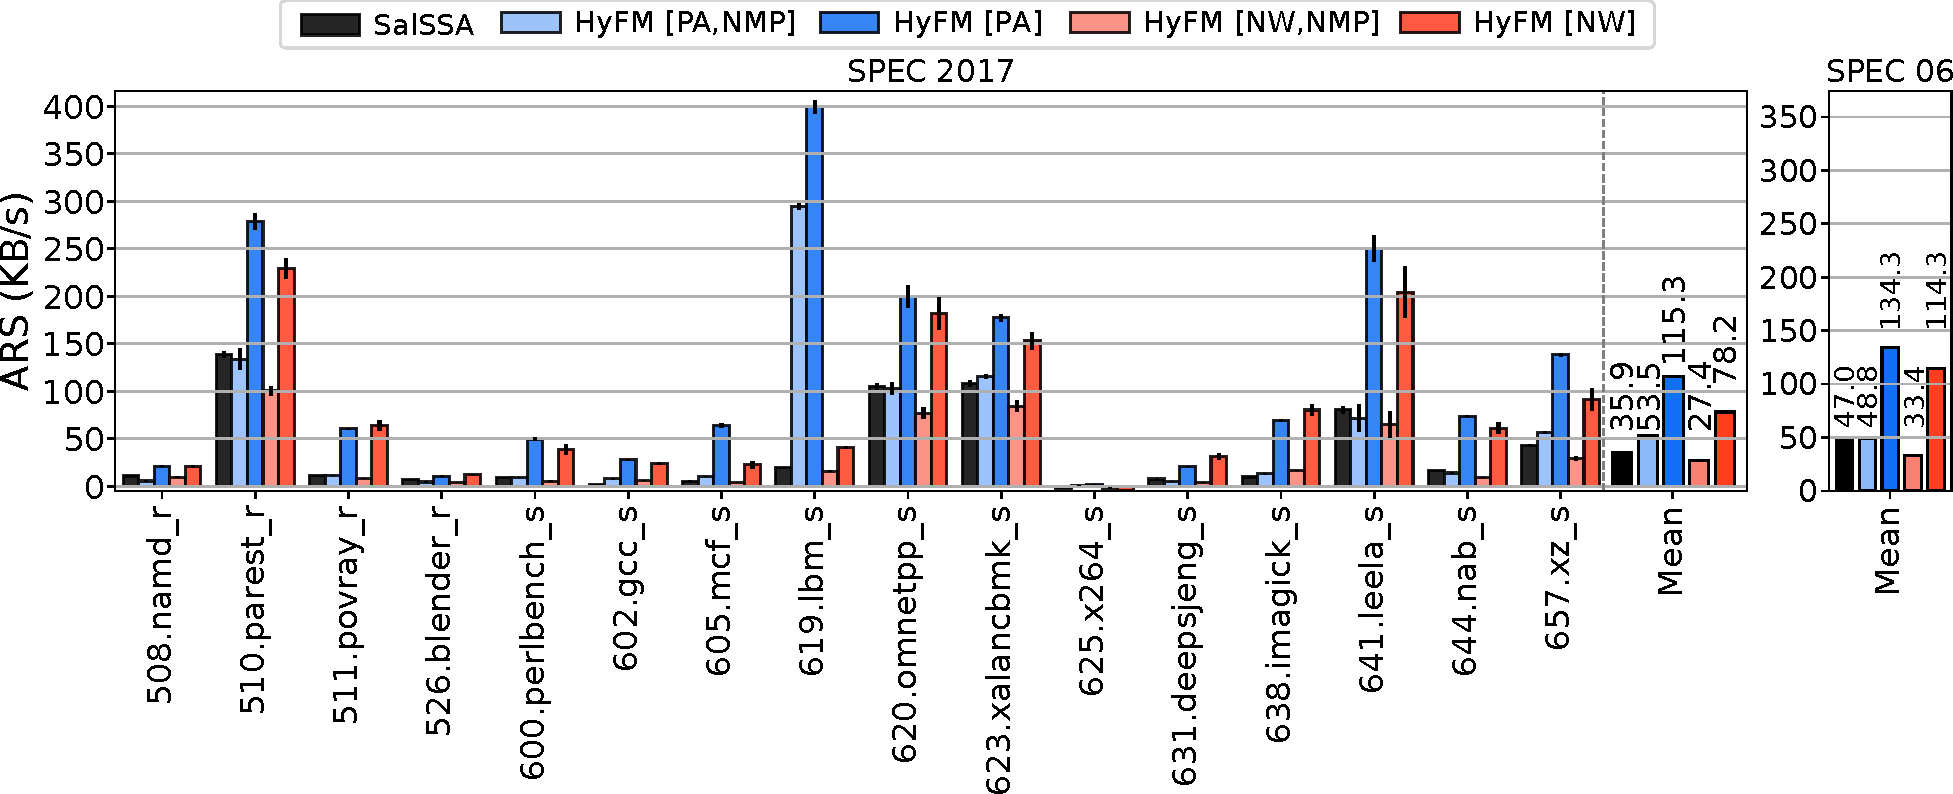
\includegraphics[width=0.95\linewidth]{src/lctes21/figs/ars-spec17-06.pdf}
%  \caption{Average reduction speed on both SPEC 2006 and 2017.}
%  \label{fig:ars-both}
%\end{figure*}

\subsection{Memory Usage} \label{sec:eval:memory}

 \begin{figure}[h]
   \centering
 \begin{subfigure}{\textwidth}
 \center
   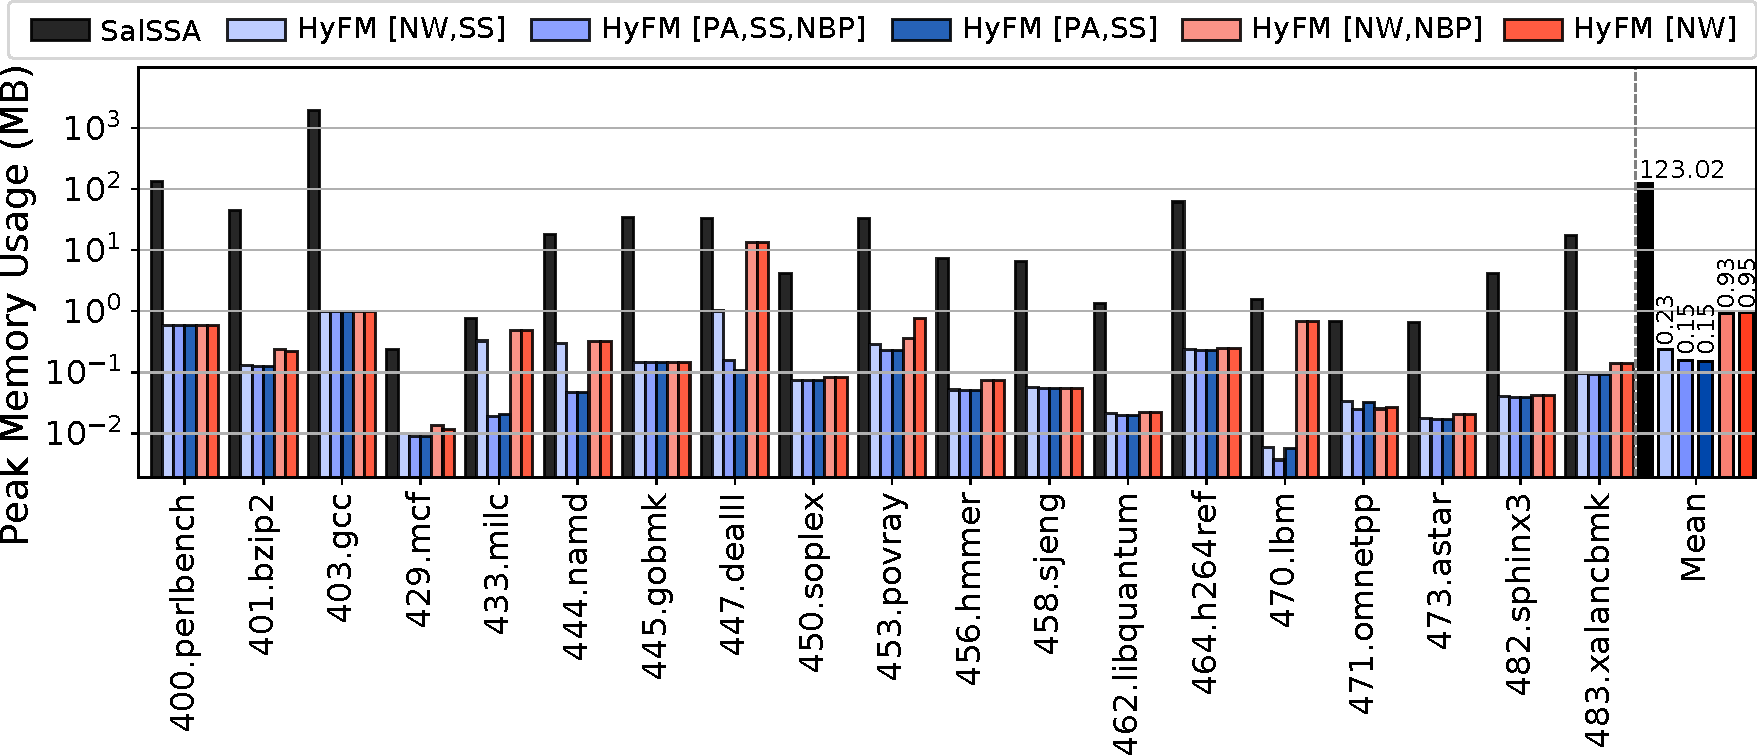
\includegraphics[width=\textwidth]{src/lctes21/figs/memory-spec06.pdf}
 \caption{SPEC CPU 2006.}
 \label{fig:memory-spec06}
 \end{subfigure}
 \\
 \begin{subfigure}{\textwidth}
 \center
   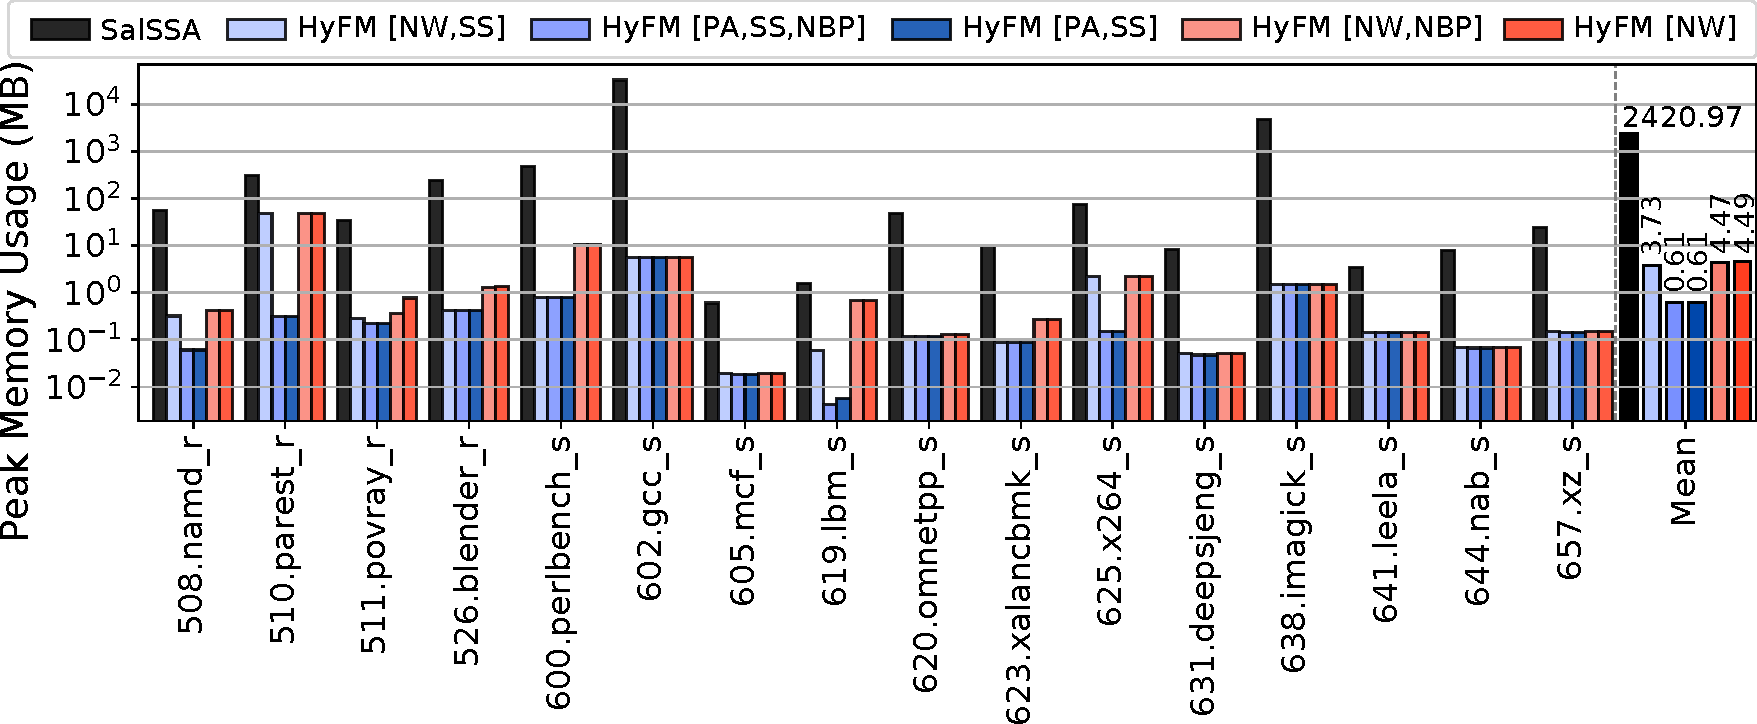
\includegraphics[width=\textwidth]{src/lctes21/figs/memory-spec17.pdf}
 \caption{SPEC CPU 2017.}
 \label{fig:memory-spec17}
 \end{subfigure}
 \caption{Peak memory usage of {\SOAName} and {\ProjName} variants for SPEC 2006 and 2017 in log scale. {\SOAName} has a peak memory usage several orders of magnitude hundreds higher than all other approaches. The pairwise alignment variants of {\ProjName} need on average only a seventh of the memory needed by the {\NW} variants.}
  \label{fig:memory-both}
 \end{figure}

%\begin{figure}[h]
%  \centering
%  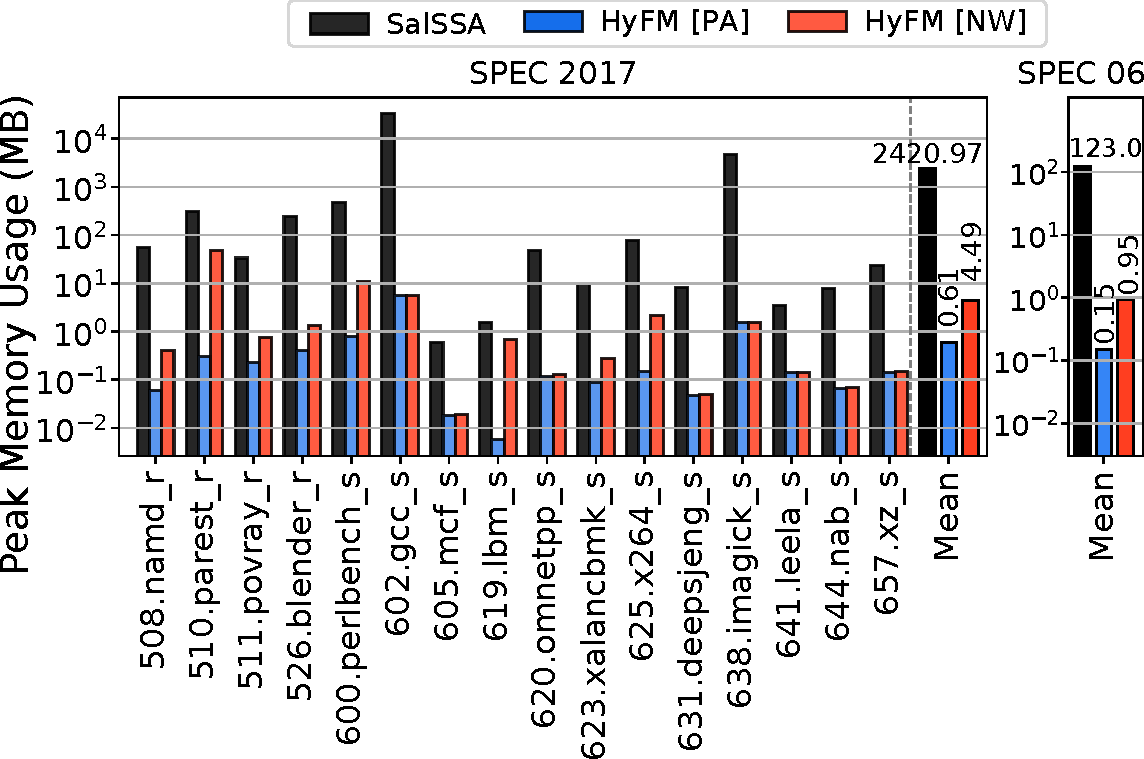
\includegraphics[width=\linewidth]{src/lctes21/figs/memory-spec17-06-tiny.pdf}
%  \caption{Peak memory usage of {\SOAName} and {\ProjName} variants for SPEC 2006 and 2017 in log scale. {\SOAName} has a peak memory usage several orders of magnitude hundreds higher than all other approaches. The pairwise alignment variants of {\ProjName} need on average only a seventh of the memory needed by the {\NW} variants.}
%  \label{fig:memory-both}
%\end{figure}

Another important aspect of function merging is peak memory usage. This is especially critical for an optimization designed for LTO.
Compilation in full LTO mode is already memory hungry. Just keeping the whole program in memory can be a significant problem for large programs~\cite{johnson17}. Maintaining additional information for every function and basic block could easily tip the compiler over the edge.

Figure~\ref{fig:memory-both} shows the peak memory usage (in log scale) needed for the alignment stage alone.
For {\SOAName}, this represents simply the execution of the {\NW} algorithm.
For {\ProjName}, the alignment stage represents both aligning each pair of basic blocks as well as the pairing these basic blocks.
Our results show that {[PA]} is over three orders of magnitude better than {\SOAName}, while {[NW]} is more than two orders of magnitude better.
In other words, while {\SOAName} requires on average 2.4~GB of memory, {[PA]} uses only around 610~KB and {[NW]} uses 5.6~MB.

The peak memory usage is especially noticeable on \texttt{gcc}, when merging its two largest functions, containing 90093 and 76265 instructions.
Since {\SOAName} applies its quadratic sequence alignment algorithm on the linearized sequences of the whole input functions, it uses over 32~GB of memory when merging these two functions.
Meanwhile, {[NW]} requires only around 5.6~MB for merging the same pair of input functions, even though it employs the same sequence alignment algorithm. This is because its peak memory usage is a quadratic function of the largest pair of \emph{blocks} instead of the largest pair of \emph{functions}.
Although very large, these two functions are composed of several thousands of very small basic blocks, so the memory overhead of {\NW} is limited.
Most of the memory consumed by {[NW]} in this case is actually needed for storing the basic block fingerprints.
This aspect becomes evident when we compare the peak memory usage of {[NW]} with that of the {[PA]} for \texttt{gcc}. They have similarly low memory requirements, even though only one of them uses a quadratic alignment algorithm.

In other cases, where basic blocks are longer, pairwise alignment leads to a significantly lower peak memory usage compared to {\NW}. For \texttt{parest}, for example, pairwise alignment reduces memory usage from \fixme{40}~MB to \fixme{200}~KB. Overall, {[PA]} needs around $6\times$ less memory. For smaller programs, {[NW]} might be a viable option but for larger ones being able to reduce memory usage to a minimum might be more important.

% \subsection{Summary}
% Overall, our novel function merging technique has surpassed the state-of-the-art in terms of compilation time, memory usage, as well as code size reduction.
% However, different variants of the proposed technique are better suited for different goals.
% If the code size is the utmost concern, {\ProjName}~[NW] is the winning strategy, but if we are looking for the most balanced trade-off between compilation-time overheads and code-size reduction, {\ProjName}~[PA] has shown better results.
